\begin{center}
\begin{tikzpicture}
	\node[anchor=south west,inner sep=0] (image)  at (0,0) {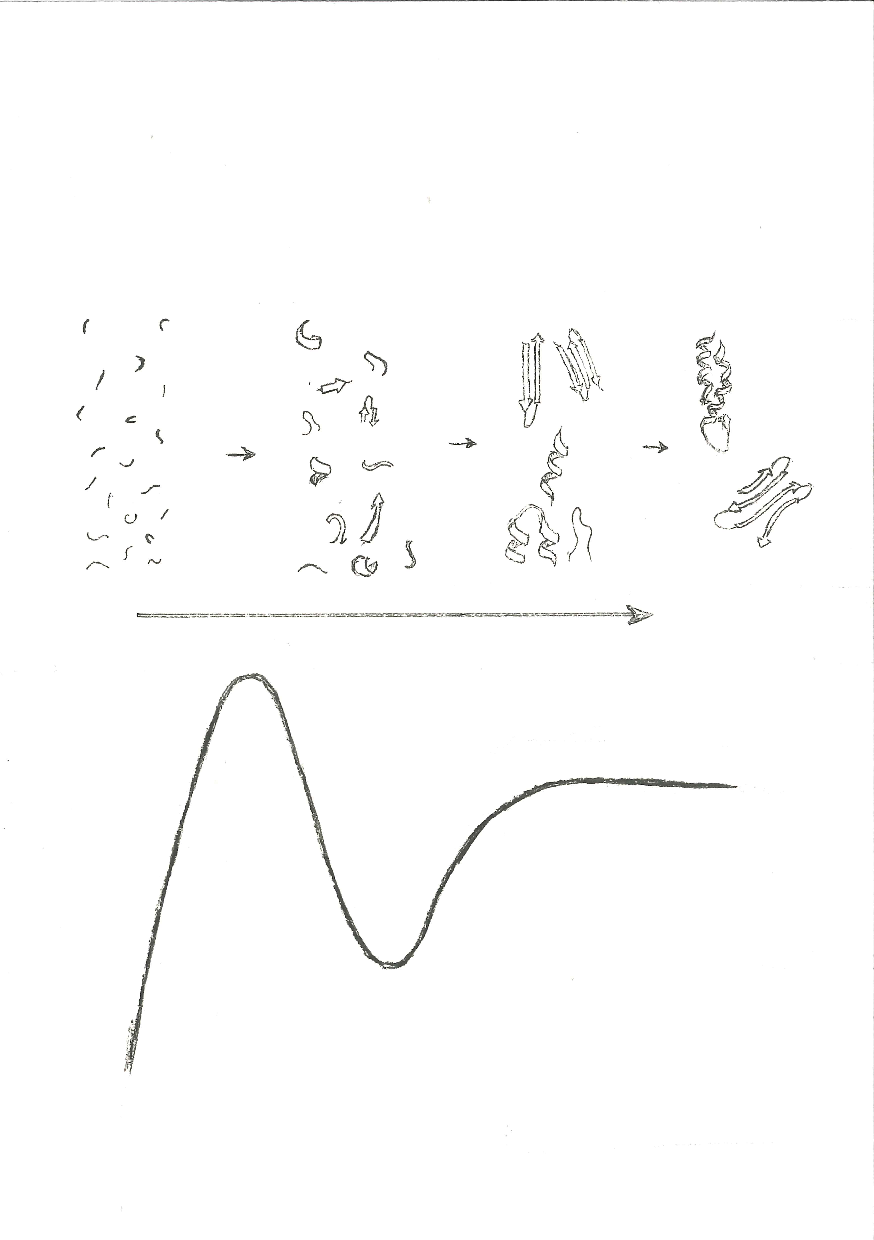
\includegraphics[trim={2mm, 2mm, 2mm, 2mm}, width=0.995\pagewidth]{scans/pan-1.pdf}};
    \begin{scope}[x={(image.south east)},y={(image.north west)}]
		\if\helplines1
			\draw[help lines,xstep=.1,ystep=.1] (0,0) grid (1,1);
		\else
			\path[help lines,xstep=.1,ystep=.1] (0,0) grid (1,1);
		\fi
		\node[text width=0.4\pagewidth, align=justify, anchor=north west] at (0.075, 0.92) {\english{In the later years there has been a revolution of \emph{deep learning}, a machine learning method where the computer looks at small bits, looks how they combine with each other in a hierarchical manner.}};
		
		\node[text width=0.4\pagewidth, align=justify, anchor=north west] at (0.075 * 1.75 + 0.4, 0.92) {\spanish{En los últimos años, el \emph{aprendizaje profundo} ha traído una revolución en este campo. En este sistema, el ordenador se fija en trozos pequeños, y en cómo se van combinando entre sí de forma jerárquica.}};
		
				
		\node(a) at (0.3, 0.47) {\english{\normalsize \emph{peak of inflated expectations}}};
		\node[below=4mm of a] {\spanish{\normalsize  \emph{pico de expectativas sobredimensionadas}}};
		
		\node[anchor=east](b) at (0.425, 0.21){\english{\normalsize \emph{abyss of disapointment}}};
		\node[right=6mm of b] {\spanish{\normalsize  \emph{ abismo de desilusión}}};
		
		\node(c) at (0.708, 0.385){\english{\normalsize \emph{plateau of productivity}}};
		\node[below=4mm of c]{\spanish{\normalsize \emph{meseta de productividad}}};
		
		\node[align=center, text width=0.8\paperwidth] at (0.5, 0.15) {\english{Gartner curve measures the cycle of hype of any new technology. Where are we in with deep learning?}};
		\node[align=center, text width=0.8\paperwidth] at (0.5, 0.07) {\spanish{La curva de Gartner mide el ciclo de sobreexcitación de las nuevas tecnologías. ¿Dónde estamos ahora con aprendizaje profundo?}};
    \end{scope}

\end{tikzpicture}
\end{center}
